\documentclass[a4paper,11pt,exos]{nsi} % COMPILE WITH DRAFT


\pagestyle{empty}
\begin{document}

%Exercice 1E12


\subsection*{NOM, Prénom : \dotfill} 

\classe{\premiere spé}
\titre{Ceinture marron 01}
\maketitle

\begin{exercice}[ : Trouver l'équation d'une parabole]
    Quelle est l'expression de la fonction polynomiale $f$ du second degré qui passe par les points de coordonnées $(-4;-29)$, $(0;-9)$ et $(4;-21)$ ?\\
    Donner la forme développée de $f$.

    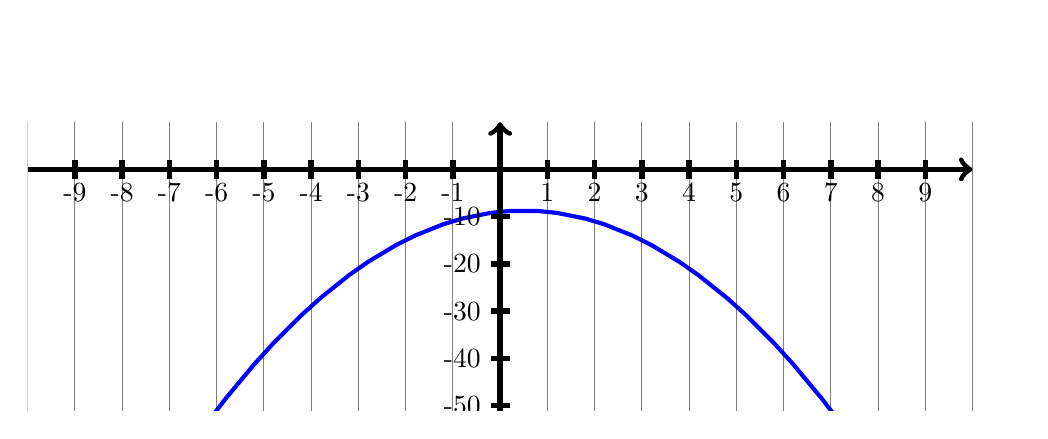
\begin{tikzpicture}[baseline, scale=0.6]
		\tikzset{ point/.style={ thick, draw, cross out, inner sep=0pt, minimum width=5pt, minimum height=5pt, }, }
		\clip (-10,-5.1) rectangle (11,3);

		\draw[color={blue}, line width=1.5];
		\draw[color={blue}, line width=1.5];
		\draw[color={blue}, line width=1.5];
		\draw[color={blue}, line width=1.5];
		\draw[color={blue}, line width=1.5];
		\draw[color={blue}, line width=1.5];
		\draw[color={blue}, line width=1.5];
		\draw[color={blue}, line width=1.5];
		\draw[color={blue}, line width=1.5];
		\draw[color={blue}, line width=1.5];
		\draw[color={blue}, line width=1.5];
		\draw[color={blue}, line width=1.5];
		\draw[color={blue}, line width=1.5];
		\draw[color={blue}, line width=1.5];
		\draw[color={blue}, line width=1.5]
			(-7.2,-6.8) --
			(-7,-6.5) --
			(-6.8,-6.2) --
			(-6.6,-5.92) --
			(-6.4,-5.64) --
			(-6.2,-5.36) --
			(-6,-5.1) --
			(-5.8,-4.84) --
			(-5.6,-4.6) --
			(-5.4,-4.36) --
			(-5.2,-4.12) --
			(-5,-3.9) --
			(-4.8,-3.68) --
			(-4.6,-3.48) --
			(-4.4,-3.28) --
			(-4.2,-3.08) --
			(-4,-2.9) --
			(-3.8,-2.72) --
			(-3.6,-2.56) --
			(-3.4,-2.4) --
			(-3.2,-2.24) --
			(-3,-2.1) --
			(-2.8,-1.96) --
			(-2.6,-1.84) --
			(-2.4,-1.72) --
			(-2.2,-1.6) --
			(-2,-1.5) --
			(-1.8,-1.4) --
			(-1.6,-1.32) --
			(-1.4,-1.24) --
			(-1.2,-1.16) --
			(-1,-1.1) --
			(-0.8,-1.04) --
			(-0.6,-1) --
			(-0.4,-0.96) --
			(-0.2,-0.92) --
			(0,-0.9) --
			(0.2,-0.88) --
			(0.4,-0.88) --
			(0.6,-0.88) --
			(0.8,-0.88) --
			(1,-0.9) --
			(1.2,-0.92) --
			(1.4,-0.96) --
			(1.6,-1) --
			(1.8,-1.04) --
			(2,-1.1) --
			(2.2,-1.16) --
			(2.4,-1.24) --
			(2.6,-1.32) --
			(2.8,-1.4) --
			(3,-1.5) --
			(3.2,-1.6) --
			(3.4,-1.72) --
			(3.6,-1.84) --
			(3.8,-1.96) --
			(4,-2.1) --
			(4.2,-2.24) --
			(4.4,-2.4) --
			(4.6,-2.56) --
			(4.8,-2.72) --
			(5,-2.9) --
			(5.2,-3.08) --
			(5.4,-3.28) --
			(5.6,-3.48) --
			(5.8,-3.68) --
			(6,-3.9) --
			(6.2,-4.12) --
			(6.4,-4.36) --
			(6.6,-4.6) --
			(6.8,-4.84) --
			(7,-5.1) --
			(7.2,-5.36) --
			(7.4,-5.64) --
			(7.6,-5.92) --
			(7.8,-6.2) --
			(8,-6.5) -- (8.2,-6.8);
		\draw[color={blue}, line width=1.5];
		\draw[color={blue}, line width=1.5];
		\draw[color={blue}, line width=1.5];
		\draw[color={blue}, line width=1.5];
		\draw[color={blue}, line width=1.5];
		\draw[color={blue}, line width=1.5];
		\draw[color={blue}, line width=1.5];
		\draw[color={blue}, line width=1.5];
		\draw[color={blue}, line width=1.5];

		\draw[color={black}, line width=2, ->] (-10,0) -- (10,0);
		\draw[color={black}, line width=2, ->] (0,-7) -- (0,1);
		\draw[color={black}, opacity=0.5] (1,-7) -- (1,1);
		\draw[color={black}, opacity=0.5] (2,-7) -- (2,1);
		\draw[color={black}, opacity=0.5] (3,-7) -- (3,1);
		\draw[color={black}, opacity=0.5] (4,-7) -- (4,1);
		\draw[color={black}, opacity=0.5] (5,-7) -- (5,1);
		\draw[color={black}, opacity=0.5] (6,-7) -- (6,1);
		\draw[color={black}, opacity=0.5] (7,-7) -- (7,1);
		\draw[color={black}, opacity=0.5] (8,-7) -- (8,1);
		\draw[color={black}, opacity=0.5] (9,-7) -- (9,1);
		\draw[color={black}, opacity=0.5] (10,-7) -- (10,1);
		\draw[color={black}, opacity=0.5] (-1,-7) -- (-1,1);
		\draw[color={black}, opacity=0.5] (-2,-7) -- (-2,1);
		\draw[color={black}, opacity=0.5] (-3,-7) -- (-3,1);
		\draw[color={black}, opacity=0.5] (-4,-7) -- (-4,1);
		\draw[color={black}, opacity=0.5] (-5,-7) -- (-5,1);
		\draw[color={black}, opacity=0.5] (-6,-7) -- (-6,1);
		\draw[color={black}, opacity=0.5] (-7,-7) -- (-7,1);
		\draw[color={black}, opacity=0.5] (-8,-7) -- (-8,1);
		\draw[color={black}, opacity=0.5] (-9,-7) -- (-9,1);
		\draw[color={black}, opacity=0.5] (-10,-7) -- (-10,1);
		\draw[color={black}, line width=2] (1,-0.2) -- (1,0.2);
		\draw[color={black}, line width=2] (2,-0.2) -- (2,0.2);
		\draw[color={black}, line width=2] (3,-0.2) -- (3,0.2);
		\draw[color={black}, line width=2] (4,-0.2) -- (4,0.2);
		\draw[color={black}, line width=2] (5,-0.2) -- (5,0.2);
		\draw[color={black}, line width=2] (6,-0.2) -- (6,0.2);
		\draw[color={black}, line width=2] (7,-0.2) -- (7,0.2);
		\draw[color={black}, line width=2] (8,-0.2) -- (8,0.2);
		\draw[color={black}, line width=2] (9,-0.2) -- (9,0.2);
		\draw[color={black}, line width=2] (-1,-0.2) -- (-1,0.2);
		\draw[color={black}, line width=2] (-2,-0.2) -- (-2,0.2);
		\draw[color={black}, line width=2] (-3,-0.2) -- (-3,0.2);
		\draw[color={black}, line width=2] (-4,-0.2) -- (-4,0.2);
		\draw[color={black}, line width=2] (-5,-0.2) -- (-5,0.2);
		\draw[color={black}, line width=2] (-6,-0.2) -- (-6,0.2);
		\draw[color={black}, line width=2] (-7,-0.2) -- (-7,0.2);
		\draw[color={black}, line width=2] (-8,-0.2) -- (-8,0.2);
		\draw[color={black}, line width=2] (-9,-0.2) -- (-9,0.2);
		\draw[color={black}, line width=2] (-0.2,-1) -- (0.2,-1);
		\draw[color={black}, line width=2] (-0.2,-2) -- (0.2,-2);
		\draw[color={black}, line width=2] (-0.2,-3) -- (0.2,-3);
		\draw[color={black}, line width=2] (-0.2,-4) -- (0.2,-4);
		\draw[color={black}, line width=2] (-0.2,-5) -- (0.2,-5);
		\draw[color={black}, line width=2] (-0.2,-6) -- (0.2,-6);
		\draw[color={black}, fill opacity=1]
			(1,-0.5)
			node[anchor=center, scale=1] {1};
		\draw[color={black}, fill opacity=1]
			(2,-0.5)
			node[anchor=center, scale=1] {2};
		\draw[color={black}, fill opacity=1]
			(3,-0.5)
			node[anchor=center, scale=1] {3};
		\draw[color={black}, fill opacity=1]
			(4,-0.5)
			node[anchor=center, scale=1] {4};
		\draw[color={black}, fill opacity=1]
			(5,-0.5)
			node[anchor=center, scale=1] {5};
		\draw[color={black}, fill opacity=1]
			(6,-0.5)
			node[anchor=center, scale=1] {6};
		\draw[color={black}, fill opacity=1]
			(7,-0.5)
			node[anchor=center, scale=1] {7};
		\draw[color={black}, fill opacity=1]
			(8,-0.5)
			node[anchor=center, scale=1] {8};
		\draw[color={black}, fill opacity=1]
			(9,-0.5)
			node[anchor=center, scale=1] {9};
		\draw[color={black}, fill opacity=1]
			(-1,-0.5)
			node[anchor=center, scale=1] {-1};
		\draw[color={black}, fill opacity=1]
			(-2,-0.5)
			node[anchor=center, scale=1] {-2};
		\draw[color={black}, fill opacity=1]
			(-3,-0.5)
			node[anchor=center, scale=1] {-3};
		\draw[color={black}, fill opacity=1]
			(-4,-0.5)
			node[anchor=center, scale=1] {-4};
		\draw[color={black}, fill opacity=1]
			(-5,-0.5)
			node[anchor=center, scale=1] {-5};
		\draw[color={black}, fill opacity=1]
			(-6,-0.5)
			node[anchor=center, scale=1] {-6};
		\draw[color={black}, fill opacity=1]
			(-7,-0.5)
			node[anchor=center, scale=1] {-7};
		\draw[color={black}, fill opacity=1]
			(-8,-0.5)
			node[anchor=center, scale=1] {-8};
		\draw[color={black}, fill opacity=1]
			(-9,-0.5)
			node[anchor=center, scale=1] {-9};
		\draw[color={black}, fill opacity=1]
			(-0.8,-1)
			node[anchor=center, scale=1] {-10};
		\draw[color={black}, fill opacity=1]
			(-0.8,-2)
			node[anchor=center, scale=1] {-20};
		\draw[color={black}, fill opacity=1]
			(-0.8,-3)
			node[anchor=center, scale=1] {-30};
		\draw[color={black}, fill opacity=1]
			(-0.8,-4)
			node[anchor=center, scale=1] {-40};
		\draw[color={black}, fill opacity=1]
			(-0.8,-5)
			node[anchor=center, scale=1] {-50};
		\draw[color={black}, fill opacity=1]
			(-0.8,-6)
			node[anchor=center, scale=1] {-60};
	\end{tikzpicture}\\
    
\end{exercice}


\carreauxseyes{16.8}{14.4}
\end{document}